\PassOptionsToPackage{unicode=true}{hyperref} % options for packages loaded elsewhere
\PassOptionsToPackage{hyphens}{url}
%
\documentclass[10pt,xcolor=table,color={dvipsnames,usenames},ignorenonframetext,usepdftitle=false,french]{beamer}
\setbeamertemplate{caption}[numbered]
\setbeamertemplate{caption label separator}{: }
\setbeamercolor{caption name}{fg=normal text.fg}
\beamertemplatenavigationsymbolsempty
\usepackage{caption}
\captionsetup{skip=0pt,belowskip=0pt}
%\setlength\abovecaptionskip{-15pt}
\usepackage{lmodern}
\usepackage{amssymb,amsmath,mathtools,multirow}
\usepackage{float,hhline}
\usepackage{tikz}
\usepackage[tikz]{bclogo}
\usepackage{mathtools}
\usepackage{ifxetex,ifluatex}
\usepackage{fixltx2e} % provides \textsubscript
\ifnum 0\ifxetex 1\fi\ifluatex 1\fi=0 % if pdftex
  \usepackage[T1]{fontenc}
  \usepackage[utf8]{inputenc}
  \usepackage{textcomp} % provides euro and other symbols
\else % if luatex or xelatex
  \usepackage{unicode-math}
  \defaultfontfeatures{Ligatures=TeX,Scale=MatchLowercase}
\fi
\usetheme[coding=utf8,language=french,
,titlepagelogo=img/LOGO-ENSAE.png
]{TorinoTh}
% use upquote if available, for straight quotes in verbatim environments
\IfFileExists{upquote.sty}{\usepackage{upquote}}{}
% use microtype if available
\IfFileExists{microtype.sty}{%
\usepackage[]{microtype}
\UseMicrotypeSet[protrusion]{basicmath} % disable protrusion for tt fonts
}{}
\IfFileExists{parskip.sty}{%
\usepackage{parskip}
}{% else
\setlength{\parindent}{0pt}
\setlength{\parskip}{6pt plus 2pt minus 1pt}
}
\usepackage{hyperref}
\hypersetup{
            pdftitle={Mastermind et permutations},
            pdfauthor={Kim Antunez, Romain Lesauvage et Alain Quartier-la-Tente},
            pdfborder={0 0 0},
            breaklinks=true}
\urlstyle{same}  % don't use monospace font for urls
\newif\ifbibliography
\usepackage{graphicx,grffile}
\makeatletter
\def\maxwidth{\ifdim\Gin@nat@width>\linewidth\linewidth\else\Gin@nat@width\fi}
\def\maxheight{\ifdim\Gin@nat@height>\textheight\textheight\else\Gin@nat@height\fi}
\makeatother
% Scale images if necessary, so that they will not overflow the page
% margins by default, and it is still possible to overwrite the defaults
% using explicit options in \includegraphics[width, height, ...]{}
\setkeys{Gin}{width=\maxwidth,height=\maxheight,keepaspectratio}
% Prevent slide breaks in the middle of a paragraph:
\widowpenalties 1 10000
\raggedbottom
\AtBeginPart{
  \let\insertpartnumber\relax
  \let\partname\relax
  \frame{\partpage}
}
\AtBeginSection{
  \ifbibliography
  \else
    \begin{frame}{Sommaire}
    \tableofcontents[currentsection, hideothersubsections]
    \end{frame}
  \fi
}
\setlength{\emergencystretch}{3em}  % prevent overfull lines
\providecommand{\tightlist}{%
  %\setlength{\itemsep}{0pt}
  \setlength{\parskip}{0pt}
  }
\setcounter{secnumdepth}{0}

% set default figure placement to htbp
\makeatletter
\def\fps@figure{htbp}
\makeatother

\usepackage{wrapfig}
\usepackage{booktabs}
\usepackage{longtable}
\usepackage{array}
\usepackage{multirow}
\usepackage[table]{xcolor}
\usepackage{wrapfig}
\usepackage{float}
\usepackage{colortbl}
\usepackage{pdflscape}
\usepackage{tabu}
\usepackage{threeparttable}
\usepackage{threeparttablex}
\usepackage[normalem]{ulem}
\usepackage{makecell}
\usepackage{animate}
\usepackage{fontawesome5}
\usepackage{caption}
\usepackage{graphicx}
\usepackage{tikz}
\usetikzlibrary{decorations}
\usetikzlibrary{decorations.pathmorphing}
\usetikzlibrary{decorations.pathreplacing}
\usetikzlibrary{decorations.shapes}
\usetikzlibrary{decorations.text}
\usetikzlibrary{decorations.markings}
\usetikzlibrary{decorations.fractals}
\usetikzlibrary{decorations.footprints}
\usepackage{hyperref}
\usepackage[T1]{fontenc}
\usepackage[utf8]{inputenc}
\usepackage{lmodern}
\usepackage{babel}

\title{Mastermind et permutations}
\ateneo{Projet Monte-Carlo, Ensae}
\author{Kim Antunez, Romain Lesauvage et Alain Quartier-la-Tente}
\date{}


\setrellabel{}

\setcandidatelabel{}

\rel{}
\division{25/04/2020}

\departement{Ensae --- 2019-2020}
\makeatletter
\let\@@magyar@captionfix\relax
\makeatother

\DeclareMathOperator{\Cov}{Cov}
\newcommand{\E}[1]{\mathbb{E}\left[ #1 \right]}
\newcommand{\V}[1]{\mathbb{V}\left[ #1 \right]}
\newcommand{\cov}[2]{\Cov\left( #1\,,\,#2 \right)}

\begin{document}
\begin{frame}[plain,noframenumbering]
\titlepage
\end{frame}

\hypertarget{introduction}{%
\section{Introduction}\label{introduction}}

\begin{frame}{Introduction}
\protect\hypertarget{introduction-1}{}

\begin{itemize}
\tightlist
\item
  \textbf{code} : \(n\) boules de couleur parmi \(m\) couleurs
  possibles\\
  (classiquement \(n = 4\) et \(m = 6\))\\
\item
  \textbf{boules noires} : boules bien placées
\item
  \textbf{boules blanches} : boules de la bonne couleur, mais mal
  placées
\end{itemize}

\begin{figure}
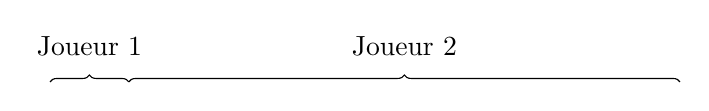
\begin{tikzpicture}
\draw[color=black,decorate,decoration={brace}] (2,2) -- (3,2) node[above=0.2cm,pos=0.5] {Joueur 1};
\draw[color=black,decorate,decoration={brace}] (3,2) -- (10,2) node[above=0.2cm,pos=0.5] {Joueur 2};
\end{tikzpicture}

\includegraphics[width=0.7\textwidth]{img/mastermind.png}
\captionsetup{margin=0cm,format=hang,justification=justified}
\end{figure}

\(\longrightarrow\) Résolution par \emph{Cross-Entropy}

\end{frame}

\hypertarget{rappels-sur-la-muxe9thode-de-cross-entropy}{%
\subsection{\texorpdfstring{Rappels sur la méthode de
\emph{Cross-Entropy}}{Rappels sur la méthode de Cross-Entropy}}\label{rappels-sur-la-muxe9thode-de-cross-entropy}}

\begin{frame}{Objectif de la \emph{Cross-Entropy}}
\protect\hypertarget{objectif-de-la-cross-entropy}{}

Résoudre \dots  \begin{equation} 
S(x^{*})=\gamma^{*}=\underset{x\in\mathcal{X}}{{\max}} S(x)
\end{equation}

\dots ~ en lui associant un problème stochastique :

\begin{itemize}
\item $1_{\left\{ S(x)\geq\gamma\right\}}$ sur $\mathcal{X}$ pour plusieurs seuils $\gamma\in\mathbb{R}$ ;  
\item $\{f(\cdot;v),\,v\in\mathcal{V}\}$ famille de probabilités sur $\mathcal{X}$, paramétrée par $v$. 
\end{itemize}

\end{frame}

\begin{frame}{Algorithme \bcoutil}
\protect\hypertarget{algorithme}{}

\begin{enumerate}

\item<1-> \textbf{Initialisation :} on fixe  $\hat{v}_{0}$, $N\in \mathbb N$ et $\rho\in]0,1[$, $t = 1$.  
\item<2-> On génère $X_{1},\dots,X_{N} \quad  {\sim} \quad f(\cdot,v_{t-1})$, on calcule 
$$\hat{\gamma}_{t}=S_{\lceil(1-\rho)N\rceil}$$

\item<3-> On utilise le même échantillon $X_{1},\dots,X_{N}$ pour trouver $\hat{v}_{t}$ :
\begin{equation}
\hat{v}_{t}=\underset{v}{argmax}\;\hat{D}(v)=\underset{v}{argmax}\frac{1}{N}\sum_{i=1}^{N}1_{\{S(X_{i})\geq\hat{\gamma}_{t}\}}\ln f(X_{i};v)
\end{equation}
\item<5->  \emph{[FACULTATIF] smoothed updating} (éviter l'occurence de 0 et de 1) :
$$
\hat{v}_{t}=\alpha\tilde{v}_{t}+(1-\alpha)\hat{v}_{t-1}
$$
\item<4-> \textbf{Arrêt} : si pour un certain $t\geq d$,  on a : 
$$\hat{\gamma}_{t}=\hat{\gamma}_{t-1}=\dots=\hat{\gamma}_{t-d}$$
\end{enumerate}

\end{frame}

\hypertarget{sec:q1}{%
\section{\texorpdfstring{Application de la méthode de
\emph{Cross-Entropy} au Mastermind
(Q1)}{Application de la méthode de Cross-Entropy au Mastermind (Q1)}}\label{sec:q1}}

\begin{frame}{Question 1 \bccrayon}
\protect\hypertarget{question-1}{}

Mettre en oeuvre un algorithme basé sur la méthode CE en détaillant :

\begin{enumerate}
\item la fonction score choisie;
\item la famille paramétrique choisie (pour simuler des codes);
\item la méthode pour simuler une loi de cette famille;
\item la méthode utilisée pour estimer le paramètre \og optimal \fg{} à chaque étape.
\end{enumerate}

\end{frame}

\hypertarget{paramuxe8tres-utilisuxe9s}{%
\subsection{Paramètres utilisés}\label{paramuxe8tres-utilisuxe9s}}

\begin{frame}{Paramètres utilisés}
\protect\hypertarget{paramuxe8tres-utilisuxe9s-1}{}

\begin{itemize}

\item<1-> $\mathcal{X}=\left\{ 1,2,\dots,m\right\}^{n}$  

\item<2-> Famille paramétrique : $$\mathcal{V} = \left\{ \left(p_{i,j}\right)_{i,j} \in\mathcal{M}_{n,m}([0,1])\::\:\forall i,\sum_{j=1}^mp_{i,j}=1\right\} $$
\textbf{Remarque} : $X=(X_{1},\dots,X_{n})\in\mathcal{X}$ tirées aléatoirement selon $p_{1},\dots,p_{n}$, la $j$ \ieme{} composante de $p_{i}$ étant égale à $p_{ij}=\mathbb{P}(X_{i}=j)$ : probabilité d'avoir une boule de couleur $j$ en $i$ème position.

\item<3-> Score : 
$$
S(x)=\frac{\omega_{noir}\times N_{\text{boules noires}}+\omega_{blanc}\times N_{\text{boules blanches}}
}{
\omega_{noir}\times n
}
$$
avec, par exemple, $\omega_{noir}=2$ et $\omega_{blanc}=1$.


\end{itemize}

\end{frame}

\hypertarget{algorithme-de-cross-entropy}{%
\subsection{\texorpdfstring{Algorithme de
\emph{Cross-Entropy}}{Algorithme de Cross-Entropy}}\label{algorithme-de-cross-entropy}}

\begin{frame}{Algorithme de \emph{Cross-Entropy}}
\protect\hypertarget{algorithme-de-cross-entropy-1}{}

\begin{enumerate}


\item Initialisation 

\begin{itemize}
\item 
\highlight{$\hat{v}_{0} = \left(\frac{1}{m}\right)_{i=1..n,j=1..m}$} (probabilités uniformes pour chaque couleur)
\item \highlight{$N = C\times m \times n $} ($C=5$ par défaut)
\item \highlight{$\rho = 0,1$} (maximisation réalisée sur les 10 \% meilleurs échantillons)

\end{itemize}
 
\item $X_{1},\dots,X_{N} \quad  {\sim} \quad f(\cdot,v_{t-1})$, 
$\hat{\gamma}_{t}=S_{\lceil(1-\rho)N\rceil}$

\item Trouver $\hat{v}_{t}$, qui correspond ici à la matrice de terme  :
\highlight{\begin{equation}
p_{k,l}=\frac{\sum_{i=1}^{N}1_{\{S(X_{i})\geq\hat{\gamma}_{t}\}}1_{\left\{ X_{i,k}=l\right\} }}{\sum_{i=1}^{N}1_{\{S(X_{i})\geq\hat{\gamma}_{t}\}}}
\end{equation}}

\item \emph{[FACULTATIF] smoothed updating}

\item Arrêt : si pour un certain $t\geq d$ (\highlight{$d = 5$}), on a : 
$\hat{\gamma}_{t}=\dots=\hat{\gamma}_{t-d}$

\end{enumerate}

\end{frame}

\hypertarget{ruxe9sultats}{%
\subsection{Résultats}\label{ruxe9sultats}}

\begin{frame}{Premiers résultats}
\protect\hypertarget{premiers-ruxe9sultats}{}

\href{https://antuki.shinyapps.io/mastermind}{Application web
interactive}

\href{https://antuki.shinyapps.io/mastermind}{\includegraphics{img/appli.png}}

\end{frame}

\begin{frame}{Résultats sur de nombreuses simulations}
\protect\hypertarget{ruxe9sultats-sur-de-nombreuses-simulations}{}

\tiny
\begin{figure}
\begin{minipage}{.4\textwidth}
\normalsize{Itération médiane

de convergence}
\end{minipage}%
\begin{minipage}{.6\textwidth}

\begin{tabular}{>{\bfseries}l|r|r|r|r|r|r|r}
\hline
\textbf{n / m } & \textbf{4} & \textbf{6} & \textbf{10} & \textbf{15} & \textbf{20} & \textbf{30} & \textbf{40}\\
\hline
4 & 8 & 8 & 9 & 10,0 & 9,5 & 10,0 & 10,0\\
\hline
6 & 9 & 10 & 11 & 11,0 & 11,0 & 11,0 & 12,0\\
\hline
10 & 11 & 12 & 13 & 13,5 & 14,0 & 14,0 & 14,0\\
\hline
15 & 12 & 13 & 15 & 16,0 & 17,0 & 17,5 & 18,0\\
\hline
20 & 13 & 14 & 16 & 18,0 & 19,5 & 19,5 & 19,5\\
\hline
30 & 14 & 16 & 19 & 21,0 & 23,0 & 24,0 & 24,0\\
\hline
40 & 16 & 17 & 19 & 22,0 & 23,0 & 27,0 & 27,0\\
\hline
\end{tabular}
\end{minipage}
\end{figure}

\begin{figure}
\begin{minipage}{.4\textwidth}
\normalsize{Nombre de simulations

n'ayant pas convergé

vers la bonne valeur}
\end{minipage}%
\begin{minipage}{.6\textwidth}

\begin{tabular}{>{\bfseries}l|r|r|r|r|r|r|r}
\hline
\textbf{n / m } & \textbf{4} & \textbf{6} & \textbf{10} & \textbf{15} & \textbf{20} & \textbf{30} & \textbf{40}\\
\hline
4 & 0 & 0 & 0 & 0 & 0 & 0 & 0\\
\hline
6 & 0 & 0 & 0 & 0 & 0 & 0 & 0\\
\hline
10 & 0 & 0 & 0 & 0 & 0 & 0 & 0\\
\hline
15 & 0 & 0 & 1 & 1 & 1 & 0 & 0\\
\hline
20 & 0 & 1 & 1 & 0 & 1 & 1 & 0\\
\hline
30 & 1 & 1 & 3 & 3 & 4 & 1 & 2\\
\hline
40 & 1 & 0 & 2 & 4 & 6 & 3 & 3\\
\hline
\end{tabular}
\end{minipage}
\end{figure}

\begin{figure}
\begin{minipage}{.4\textwidth}
\normalsize{Moyenne de l'erreur

à la simulation

de convergence}
\end{minipage}%
\begin{minipage}{.6\textwidth}

\begin{tabular}{>{\bfseries}l|r|r|r|r|r|r|r}
\hline
\textbf{n / m } & \textbf{4} & \textbf{6} & \textbf{10} & \textbf{15} & \textbf{20} & \textbf{30} & \textbf{40}\\
\hline
4 & 0,000 & 0,000 & 0,000 & 0,000 & 0,000 & 0,000 & 0,000\\
\hline
6 & 0,000 & 0,000 & 0,000 & 0,000 & 0,000 & 0,000 & 0,000\\
\hline
10 & 0,000 & 0,000 & 0,000 & 0,000 & 0,000 & 0,000 & 0,000\\
\hline
15 & 0,000 & 0,000 & 0,003 & 0,003 & 0,003 & 0,000 & 0,000\\
\hline
20 & 0,000 & 0,005 & 0,005 & 0,000 & 0,005 & 0,005 & 0,000\\
\hline
30 & 0,003 & 0,003 & 0,010 & 0,005 & 0,008 & 0,002 & 0,007\\
\hline
40 & 0,003 & 0,000 & 0,005 & 0,005 & 0,009 & 0,004 & 0,004\\
\hline
\end{tabular}
\end{minipage}
\end{figure}

\begin{figure}
\begin{minipage}{.4\textwidth}
\normalsize{Moyenne du temps de

calcul jusqu'à

la convergence}
\end{minipage}%
\begin{minipage}{.6\textwidth}

\begin{tabular}{>{\bfseries}l|r|r|r|r|r|r|r}
\hline
\textbf{n / m } & \textbf{4} & \textbf{6} & \textbf{10} & \textbf{15} & \textbf{20} & \textbf{30} & \textbf{40}\\
\hline
4 & 0 & 0 & 0 & 0 & 0 & 0 & 0\\
\hline
6 & 0 & 0 & 0 & 0 & 0 & 1 & 1\\
\hline
10 & 0 & 0 & 1 & 1 & 1 & 2 & 3\\
\hline
15 & 0 & 1 & 1 & 2 & 3 & 6 & 8\\
\hline
20 & 1 & 1 & 2 & 4 & 6 & 11 & 16\\
\hline
30 & 1 & 3 & 6 & 11 & 17 & 30 & 43\\
\hline
40 & 3 & 5 & 11 & 21 & 31 & 60 & 88\\
\hline
\end{tabular}

\end{minipage}
\end{figure}

\normalsize

\end{frame}

\hypertarget{restriction-aux-permutations-q2}{%
\section{Restriction aux permutations
(Q2)}\label{restriction-aux-permutations-q2}}

\begin{frame}{Question 2 \bccrayon}
\protect\hypertarget{question-2}{}

Le Joueur 1 choisit obligatoirement une \textbf{permutation} (chaque
couleur ne peut apparaître qu'une seule fois, donc \(m \geq n\)).

\begin{enumerate}
\item  Mettre en oeuvre l’algorithme précédent en l'adaptant ;
\item  La méthode d’estimation utilisée dans la question précédente
est toujours valide ? 
\end{enumerate}

\end{frame}

\hypertarget{adaptation-de-lalgorithme-pruxe9cuxe9dent}{%
\subsection{Adaptation de l'algorithme
précédent}\label{adaptation-de-lalgorithme-pruxe9cuxe9dent}}

\begin{frame}{Adaptation du mécanisme de génération\dots}
\protect\hypertarget{adaptation-du-muxe9canisme-de-guxe9nuxe9ration}{}

Par rapport à l'algorithme précédent, on ne change que le
\textbf{mécanisme de génération} des échantillons :

\pause

Les échantillons sont désormais générés grâce à une loi \og sans remise
\fg{}.

\begin{itemize}
\item Initialisation : on tire la première boule, entier $x_1$, selon la loi discrète donnée par $p_{1,\cdot} = (p_{1,1},\dots, p_{1,m})$. On pose $k=1$ et $P^{(1)} = P$.
\pause
\item Itération : $P^{(k+1)}$ est obtenue en remplaçant la colonne $k$ de $P^{(k)}$ par 0 et en normalisant les lignes (somme = 1). On tire $x_{k+1}$ selon la loi discrète donnée par la ligne $k+1$ de $P^{(k+1)}$. 
\pause
\item Si $k=n$ alors on arrête, sinon on pose $k=k+1$ et on répéte l'étape 2.
\end{itemize}

\end{frame}

\begin{frame}{\dots ~Mais la méthode d'estimation reste la même}
\protect\hypertarget{mais-la-muxe9thode-destimation-reste-la-muxeame}{}

Les \(p_{k,l}\) s'interprètent de la même façon qu'en question 1 et la
formule de mise à jour des paramètres s'écrit : \[p_{k,l}=\frac{
\sum_{i=1}^{N}1_{\{S(X_{i})\geq\hat{\gamma}_{t}\}}1_{\left\{ X_{i,k}=l\right\} }
\highlight{1_{\{X_{i}\text{ permutation}\}}}
}{
\sum_{i=1}^{N}1_{\{S(X_{i})\geq\hat{\gamma}_{t}\}}
\highlight{1_{\{X_{i}\text{ permutation}\}}}
}\]

\pause

Possibilité d'appliquer la méthode de génération des échantillons de la
\textbf{question 1} \dots

\pause

\dots ~mais dans ce cas, beaucoup d'échantillons non pertinents (les
non-permutations)

\pause

\(\longrightarrow\) Algorithme de la \textbf{question 2} améliore le
processus en ne conservant que les permutations (telles que
\(1_{\{X_{i}\text{ permutation}\}} = 1\))

\end{frame}

\hypertarget{ruxe9sultats-1}{%
\subsection{Résultats}\label{ruxe9sultats-1}}

\begin{frame}{Résultats}
\protect\hypertarget{ruxe9sultats-2}{}

\tiny
\begin{figure}
\begin{minipage}{.4\textwidth}
\normalsize{Itération médiane

de convergence

\faArrowCircleRight \textbf{\ converge + vite\dots}
}
\end{minipage}%
\begin{minipage}{.6\textwidth}

\begin{tabular}{>{\bfseries}l|r|r|r|r|r|r|r}
\hline
\textbf{n / m } & \textbf{4} & \textbf{6} & \textbf{10} & \textbf{15} & \textbf{20} & \textbf{30} & \textbf{40}\\
\hline
4 & 7 & 8 & 9,0 & 9 & 9 & 10 & 10\\
\hline
6 &  & 8 & 9,5 & 10 & 10 & 11 & 11\\
\hline
10 &  &  & 10,0 & 12 & 12 & 13 & 13\\
\hline
15 &  &  &  & 12 & 14 & 15 & 15\\
\hline
20 &  &  &  &  & 14 & 17 & 17\\
\hline
30 &  &  &  &  &  & 18 & 19\\
\hline
40 &  &  &  &  &  &  & 21\\
\hline
\end{tabular}
\end{minipage}
\end{figure}

\begin{figure}
\begin{minipage}{.4\textwidth}
\normalsize{Nombre de simulations

n'ayant pas convergé

vers la bonne valeur}
\end{minipage}%
\begin{minipage}{.6\textwidth}

\begin{tabular}{>{\bfseries}l|r|r|r|r|r|r|r}
\hline
\textbf{n / m } & \textbf{4} & \textbf{6} & \textbf{10} & \textbf{15} & \textbf{20} & \textbf{30} & \textbf{40}\\
\hline
4 & 0 & 0 & 0 & 0 & 0 & 0 & 0\\
\hline
6 &  & 0 & 0 & 0 & 0 & 0 & 0\\
\hline
10 &  &  & 0 & 0 & 0 & 0 & 0\\
\hline
15 &  &  &  & 0 & 0 & 0 & 0\\
\hline
20 &  &  &  &  & 0 & 0 & 0\\
\hline
30 &  &  &  &  &  & 0 & 0\\
\hline
40 &  &  &  &  &  &  & 0\\
\hline
\end{tabular}
\end{minipage}
\end{figure}

\begin{figure}
\begin{minipage}{.4\textwidth}
\normalsize{Moyenne de l'erreur

à la simulation

de convergence
}
\end{minipage}%
\begin{minipage}{.6\textwidth}

\begin{tabular}{>{\bfseries}l|r|r|r|r|r|r|r}
\hline
\textbf{n / m } & \textbf{4} & \textbf{6} & \textbf{10} & \textbf{15} & \textbf{20} & \textbf{30} & \textbf{40}\\
\hline
4 & 0 & 0 & 0 & 0 & 0 & 0 & 0\\
\hline
6 &  & 0 & 0 & 0 & 0 & 0 & 0\\
\hline
10 &  &  & 0 & 0 & 0 & 0 & 0\\
\hline
15 &  &  &  & 0 & 0 & 0 & 0\\
\hline
20 &  &  &  &  & 0 & 0 & 0\\
\hline
30 &  &  &  &  &  & 0 & 0\\
\hline
40 &  &  &  &  &  &  & 0\\
\hline
\end{tabular}
\end{minipage}
\end{figure}

\begin{figure}
\begin{minipage}{.4\textwidth}
\normalsize{Moyenne du temps de calcul

jusqu'à la convergence

\faArrowCircleRight \textbf{\ \dots \ mais est + gourmand}
}
\end{minipage}%
\begin{minipage}{.6\textwidth}

\begin{tabular}{>{\bfseries}l|r|r|r|r|r|r|r}
\hline
\textbf{n / m } & \textbf{4} & \textbf{6} & \textbf{10} & \textbf{15} & \textbf{20} & \textbf{30} & \textbf{40}\\
\hline
4 & 0 & 0 & 0 & 0 & 0 & 1 & 1\\
\hline
6 &  & 0 & 0 & 1 & 1 & 2 & 3\\
\hline
10 &  &  & 1 & 2 & 3 & 6 & 9\\
\hline
15 &  &  &  & 5 & 9 & 15 & 22\\
\hline
20 &  &  &  &  & 15 & 29 & 44\\
\hline
30 &  &  &  &  &  & 69 & 109\\
\hline
40 &  &  &  &  &  &  & 211\\
\hline
\end{tabular}
\end{minipage}
\end{figure}

\normalsize

\end{frame}

\hypertarget{loi-spuxe9cifique-pour-guxe9nuxe9rer-les-permutations-q3}{%
\section{Loi spécifique pour générer les permutations
(Q3)}\label{loi-spuxe9cifique-pour-guxe9nuxe9rer-les-permutations-q3}}

\hypertarget{application-de-lalgorithme-de-ce}{%
\subsection{Application de l'algorithme de
CE}\label{application-de-lalgorithme-de-ce}}

\begin{frame}{Question 3 \bccrayon}
\protect\hypertarget{question-3}{}

Considérons désormais la loi suivante sur l'ensemble des permutations :
\[\pi_{\lambda,x^*}(x) \propto \exp{(-\lambda d(x,x^{*}))}\] avec :

\begin{itemize}
\item $\lambda$ > 0
\item $d(x,x^{*})$ : distance de Hamming (nombre de positions où les deux permutations $x$ et $x^{*}$ diffèrent). 
\end{itemize}

\begin{enumerate}
\item Proposer un algorithme de MCMC pour simuler selon une telle loi ;
\item Utiliser cet algorithme au sein d’une approche CE ;
\item Comparer la performance de l’algorithme obtenu à l’algorithme proposé en question 1.
\end{enumerate}

\end{frame}

\begin{frame}{Adaptation de l'algorithme de CE}
\protect\hypertarget{adaptation-de-lalgorithme-de-ce}{}

\begin{enumerate}


\item Initialisation 

\begin{itemize}
\item 
\highlight{Tirage aléatoire de $x^*_0$ et  $\lambda_0=1$.}
\item $N = C\times \highlight{(n+1)} $ ($C=5$ par défaut)
\item $\rho = 0,1$ (maximisation réalisée sur les 10 \% meilleurs échantillons)

\end{itemize}
 
\item $X_{1},\dots,X_{N}$ générés avec la \highlight{loi $\pi_{\lambda_t,x^*_t}$} (Metropolis-Hastings), calcul de 
$\hat{\gamma}_{t}=S_{\lceil(1-\rho)N\rceil}$

\item \highlight{Trouver $\tilde x_{t+1}$. Si $S(\tilde x_{t+1})\geq S(x^*_t)$ alors $x^*_{t+1} = \tilde x_{t+1}$, sinon $x^*_{t+1}=x^*_{t}$. On fixe $\lambda_{t+1}=1$}

\item \emph{[FACULTATIF] \highlight{Pas de smoothed updating}}

\item \highlight{Arrêt : si pour un certain $t$, $S(x^*_{t})=1$ alors on arrête l'algorithme.}

\end{enumerate}

\end{frame}

\hypertarget{guxe9nuxe9ration-des-donnuxe9es}{%
\subsection{Génération des
données}\label{guxe9nuxe9ration-des-donnuxe9es}}

\begin{frame}{Génération de l'échantillon : Metropolis-Hastings}
\protect\hypertarget{guxe9nuxe9ration-de-luxe9chantillon-metropolis-hastings}{}

\faArrowCircleRight \textbf{ mécanisme de proposition} : inverser deux
éléments de la permutation (symétrique).

\pause

Pour
\only<2-6>{$\boldsymbol{m=n}$ (vraies permutations) }\only<7->{$\highlight{\boldsymbol{m>n}}$}

\begin{itemize}
\item Initialisation : on choisit $x_0$ une permutation au hasard et on fixe $t=0$.

\pause 

\item Itération : 
\begin{itemize}
\item On permute au hasard deux éléments $i$ et $j$ de $x_t$ et on note $x'$ la nouvelle permutation. \only<7->{$\highlight{\rightarrow\;i\text{ ou }j \leq n}$}

\pause 

\item On calcule la probabilité d'acceptation : $r(x',x_t)=\min\left(1,\,\frac{\pi_{\lambda,x^*}(x')}{\pi_{\lambda,x^*}(x_{t})}\right)
=\min\left(1,\,\mathrm{e^{-\lambda(d(x',x^{*})-d(x_{t},x^{*}))}}\right)$  

 \onslide<7->{$\highlight{\rightarrow}$ \highlight{distances calculées sur} $\highlight{n}$ \highlight{premières coordonnées}}

\pause 

\item Acceptation ou rejet : on génére une loi uniforme $u\in[0,1]$. Si $u \leq r(x',x_{t}) $ alors on accepte le nouvel état et on pose $x_{t+1}=x'$, sinon $x_{t+1}=x_{t}$.

\pause 

\item Incrémentation : $t=t+1$.
\end{itemize}
\end{itemize}

\end{frame}

\begin{frame}{Génération de l'échantillon : Metropolis-Hastings}
\protect\hypertarget{guxe9nuxe9ration-de-luxe9chantillon-metropolis-hastings-1}{}

\textbf{Remarque} : Pour \(\lambda\) grand on converge vers \(x^*\) et
tous les échantillons seront égaux à \(x^*\).

\bigskip
\bigskip

\pause

L'algorithme de Metropolis-Hastings a \textbf{deux désavantages} :

\begin{enumerate}
\item Le \emph{burn-in}.
\item Les échantillons générés à des périodes proches sont corrélés entre eux. 
\end{enumerate}

\end{frame}

\begin{frame}{Gestion du burn-in}
\protect\hypertarget{gestion-du-burn-in}{}

\begin{figure}
\begin{minipage}{.5\textwidth}
\includegraphics[width=1\textwidth]{img/n_4_m_6.png}
\captionsetup{margin=0cm,format=hang,justification=justified}
\caption{n = 4, m = 6}
\end{minipage}%
\begin{minipage}{.5\textwidth}
\includegraphics[width=1\textwidth]{img/n_40_m_40.png}
\captionsetup{margin=0cm,format=hang,justification=justified}
\caption{n = 40, m = 40}
\end{minipage}
\end{figure}

\bigskip

\bigskip

\(\longrightarrow\) Enlever les \(250\times m\) premières observations.

\end{frame}

\begin{frame}{Gestion des autocorrélations}
\protect\hypertarget{gestion-des-autocorruxe9lations}{}

Autocorrélogrammes des 4 premières composantes des échantillons
(\(\lambda = 1\), \(n = 10\) et \(m = 40\))

\begin{figure}
\begin{minipage}{.5\textwidth}
\includegraphics[width=1\textwidth]{img/acfn10m40.png}
\captionsetup{margin=0cm,format=hang,justification=justified}
\caption{Toutes les autocorrélations}
\end{minipage}%
\begin{minipage}{.5\textwidth}
\includegraphics[width=1\textwidth]{img/acfn10m40corr.png}
\captionsetup{margin=0cm,format=hang,justification=justified}
\caption{Pas de 80 périodes}
\end{minipage}
\end{figure}

\bigskip

\(\longrightarrow\) Conserver uniquement les simulations séparées de
\(t = 80\) périodes.

\(\longrightarrow\) Intégrer ce test dans le mécanisme de proposition
est \textbf{très couteux en temps}.

\end{frame}

\begin{frame}{Estimation de \(x^*\)}
\protect\hypertarget{estimation-de-x}{}

\bcloupe (Arrieta, 2014) montre qu'on peut séparer le problème
d'estimation de \(x^*\) et \(\lambda\)

\pause

Trouver le \(x^*\) qui minimise la somme
\(\sum_{i=1}^N 1_{\{S(X_{i})\geq\hat{\gamma}_{t}\}}d(X_i,x^*)\)

\begin{itemize}

\pause 

\item Intuitivement, il s'agit de $x^*=(x_1^*,\dots,x_n^*)$ tel que $x_j^*$ correspond au chiffre le plus fréquent dans la $j$ème coordonnée des 10 % meilleurs échantillons.

\pause 

\item On part de ce principe en imposant que $x^*$ soit bien une permutation :

\begin{enumerate}
\item On crée une matrice $F=(f_{i,j})\in\mathcal M_{n,m}(\mathbb{N})$ telle $f_{i,j}$ soit égal au nombre de fois que l'entier $j$ apparait en $i$ème position parmi les 10 % meilleurs échantillon.

\item On sélectionne une composante par ligne et par colonne de $F$ de façon à ce que leur somme soit maximale
\end{enumerate}
\end{itemize}

\end{frame}

\begin{frame}{Estimation de \(\lambda\)}
\protect\hypertarget{estimation-de-lambda}{}

Plusieurs tests réalisés pour estimer \(\lambda\) :

\begin{enumerate}
\item croissance linéaire à chaque itération
\item constance

\pause 

\item (Arrieta, 2014) nous fournit la constante de normalisation de $\pi_{\lambda,x^*}$ :
$$
m!\exp(-\lambda m)\sum_{k=0}^{m}\frac{(\exp(\lambda)-1)^{k}}{k!}
$$

le $\lambda$ qui maximise la vraisemblance est alors tel que :
\footnotesize
$$
\frac{
\exp(\lambda)\sum_{k=0}^{m-1}\frac{(\exp(\lambda)-1)^{k}}{k!} -
m\sum_{k=0}^{m}\frac{(\exp(\lambda)-1)^{k}}{k!}
}{
\sum_{k=0}^{m}\frac{(\exp(\lambda)-1)^{k}}{k!}
} +
\frac{\sum_{i=1}^N 1_{\{S(X_{i})\geq\hat{\gamma}_{t}\}}d(X_i,x^*)}{\sum_{i=1}^N 1_{\{S(X_{i})\geq\hat{\gamma}_{t}\}}} = 0
$$
\normalsize

\textbf{Problème} : croissance rapide de $\lambda$ à chaque itération. Si $y$ n'est pas décodé dans les premières itérations, les échantillons $X_i$ générés seront très proches de $x^*$ et on ne trouvera pas $y$.
\end{enumerate}

\pause

\textbf{$\longrightarrow$ Meilleure solution : $\lambda = 1$.}

\end{frame}

\hypertarget{ruxe9sultats-3}{%
\subsection{Résultats}\label{ruxe9sultats-3}}

\begin{frame}{Résultats}
\protect\hypertarget{ruxe9sultats-4}{}

\tiny
\begin{figure}
\begin{minipage}{.4\textwidth}
\normalsize{Itération médiane

de convergence

\faArrowCircleRight \textbf{\ converge - vite}
}
\end{minipage}%
\begin{minipage}{.6\textwidth}

\begin{tabular}{>{\bfseries}l|r|r|r|r|r|r|r}
\hline
\textbf{n / m } & \textbf{4} & \textbf{6} & \textbf{10} & \textbf{15} & \textbf{20} & \textbf{30} & \textbf{40}\\
\hline
4 & 14,5 & 4 & 8,5 & 17 & 25,5 & 21,5 & 91\\
\hline
6 &  & 6 & 15,0 & 19 & 90,0 &  & \\
\hline
10 &  &  & 9,0 & 31 & 73,5 &  & \\
\hline
15 &  &  &  & 14 & 49,0 &  & \\
\hline
20 &  &  &  &  & 23,0 &  & \\
\hline
30 &  &  &  &  &  & 95,0 & \\
\hline
40 &  &  &  &  &  &  & \\
\hline
\end{tabular}
\end{minipage}
\end{figure}

\begin{figure}
\begin{minipage}{.4\textwidth}
\normalsize{Nombre de simulations

n'ayant pas convergé

vers la bonne valeur

\faArrowCircleRight \textbf{\ converge - souvent}
}
\end{minipage}%
\begin{minipage}{.6\textwidth}

\begin{tabular}{>{\bfseries}l|r|r|r|r|r|r|r}
\hline
\textbf{n / m } & \textbf{4} & \textbf{6} & \textbf{10} & \textbf{15} & \textbf{20} & \textbf{30} & \textbf{40}\\
\hline
4 & 0 & 0 & 0 & 0 & 4 & 8 & 6\\
\hline
6 &  & 0 & 0 & 2 & 6 & 10 & 10\\
\hline
10 &  &  & 0 & 3 & 6 & 10 & 10\\
\hline
15 &  &  &  & 0 & 7 & 10 & 10\\
\hline
20 &  &  &  &  & 0 & 10 & 10\\
\hline
30 &  &  &  &  &  & 7 & 10\\
\hline
40 &  &  &  &  &  &  & 10\\
\hline
\end{tabular}

\end{minipage}
\end{figure}

\begin{figure}
\begin{minipage}{.4\textwidth}
\normalsize{Moyenne de l'erreur

à la simulation

de convergence
}
\end{minipage}%
\begin{minipage}{.6\textwidth}

\begin{tabular}{>{\bfseries}l|r|r|r|r|r|r|r}
\hline
\textbf{n / m } & \textbf{4} & \textbf{6} & \textbf{10} & \textbf{15} & \textbf{20} & \textbf{30} & \textbf{40}\\
\hline
4 & 0,025 & 0,312 & 0,462 & 0,525 & 0,550 & 0,662 & 0,725\\
\hline
6 &  & 0,208 & 0,425 & 0,492 & 0,567 & 0,633 & 0,725\\
\hline
10 &  &  & 0,295 & 0,440 & 0,530 & 0,640 & 0,700\\
\hline
15 &  &  &  & 0,360 & 0,460 & 0,587 & 0,667\\
\hline
20 &  &  &  &  & 0,385 & 0,528 & 0,622\\
\hline
30 &  &  &  &  &  & 0,425 & 0,535\\
\hline
40 &  &  &  &  &  &  & 0,450\\
\hline
\end{tabular}
\end{minipage}
\end{figure}

\begin{figure}
\begin{minipage}{.4\textwidth}
\normalsize{Moyenne du temps de calcul

jusqu'à la convergence

\faArrowCircleRight \textbf{\ et est + gourmand}
}
\end{minipage}%
\begin{minipage}{.6\textwidth}

\begin{tabular}{>{\bfseries}l|r|r|r|r|r|r|r}
\hline
\textbf{n / m } & \textbf{4} & \textbf{6} & \textbf{10} & \textbf{15} & \textbf{20} & \textbf{30} & \textbf{40}\\
\hline
4 & 1 & 0 & 2 & 4 & 6 & 5 & 26\\
\hline
6 &  & 1 & 3 & 5 & 19 &  & \\
\hline
10 &  &  & 2 & 10 & 15 &  & \\
\hline
15 &  &  &  & 5 & 18 &  & \\
\hline
20 &  &  &  &  & 12 &  & \\
\hline
30 &  &  &  &  &  & 64 & \\
\hline
40 &  &  &  &  &  &  & \\
\hline
\end{tabular}
\end{minipage}
\end{figure}

\normalsize

\end{frame}

\begin{frame}{Merci pour votre attention}
\protect\hypertarget{merci-pour-votre-attention}{}

\href{https://github.com/ARKEnsae/Mastermind_Simulation}{\faGithub{} ARKEnsae/Mastermind\_Simulation}

\href{https://antuki.shinyapps.io/mastermind}{\faChartBar{} Application web}

\href{https://arkensae.github.io/Mastermind_Simulation/Rapport/Rapport.html}{\faEdit{} Rapport du projet}

\begin{center}
\includegraphics[width = 2.5cm]{img/LOGO-ENSAE.png}
\end{center}

\end{frame}

\end{document}
